%!TEX root = ../thesis-main.tex

\chapter{Introduzione}\label{chap:introduction}
Il mondo del software ha scritto diverse decadi di storia. Sin dagli anni '50, quando i primi calcolatori programmabili hanno fatto il loro ingresso sul mercato, il software ha assunto un ruolo sempre più pervasivo nella vita quotidiana delle persone. Oltre ad essere parte integrante dei sistemi informativi delle aziende, lo possiamo trovare anche all'interno di automobili, elettrodomestici e tantissimi strumenti con la quale abbiamo a che fare nella nostra quotidianità. La crescente diffusione del software ha introdotto la necessità di progettare metodologie di sviluppo solide e versatili. Uno dei primi è il \textbf{modello a cascata} il quale struttura il processo di realizzazione del software in fasi sequenziali lineari. Il modello riprende la tipica organizzazione della produzione manifatturiera e fu progressivamente abbandonato con l'evolversi delle richieste del mercato. Successivamente prese piede il concetto di modelli iterativi come il \textbf{modello a spirale} in cui il processo di sviluppo è suddiviso in fasi multiple ripetute più volte (iterazioni). Gli ultimi decenni hanno dato vita a un nuovo modello, considerato lo standard dell'industria, la \textbf{metodologia agile}. Quest'ultima non rappresenta un unico modello, ma un insieme di modelli iterativi costruiti sulla base dei principi definiti all'interno del manifesto agile. Questi principi mettono in primo piano un ambiente autonomo e dinamico in cui sono fondamentali: cicli di sviluppo brevi, continui miglioramenti, la comunicazione col cliente e la consegna tempestiva di funzionalità. Il progetto esposto in questo documento introduce un evoluzione del concetto agile nato recentemente nel mondo dello sviluppo del software, conosciuto come ``DevOps".

\section{Contesto}
Con l'avvento di internet il concetto di software come un entità sviluppata e finita ha completamente cessato di esistere. Mediante la rete è diventato semplice ed efficiente distribuire un programma e fornire un ulteriore supporto attraverso aggiornamenti evolutivi e correttivi. Il fenomeno è cresciuto tanto da aver dato luce alla pratica del rilascio di applicazioni deliberatamente non complete, le quali attraverso il feedback degli utenti evolvono verso un prodotto finito. Il manifesto agile ha introdotto la cultura di emettere frequenti rilasci di nuove versioni del software, rendendo la distribuzione un punto cardine all'interno del ciclo di vita di esso. Dietro lo sviluppo rapido di nuove funzionalità è necessario il rilascio di queste altrettanto velocemente, la filosofia DevOps nasce per soddisfare questa esigenza.

\subsection{DevOps}
La metodologia DevOps (termine nato dalla contrazione di ``Development" ed ``Operations") si è formata intorno al 2008 con l'idea chiave di unire il team di sviluppo ed il team operativo. Il principale catalizzatore di questo concetto è stata la necessità di affrontare inefficienze nelle fasi del ciclo di vita del software. Differentemente dalla metodologia agile, DevOps è una filosofia di sviluppo software che esprime attraverso tre pilastri il suo obiettivo:

\begin{itemize}
	\item il \textbf{flusso}, il miglioramento del flusso di lavoro lungo l'intero processo di produzione, ciò significa ottimizzare il processo dall'idea, fino alla generazione di valore con il software in produzione.
	\item Il \textbf{feedback}, mediante cicli di feedback rapidi si garantisce la scoperta di difetti nel codice nelle fasi iniziali del ciclo di vita del prodotto. Ciò comporta rapide correzioni, minor debito tecnico e la garanzia di possedere in qualsiasi momento un software stabile e qualitativamente pronto ad un rilascio.
	\item L'\textbf{apprendimento continuo}, la filosofia DevOps promuove la sperimentazione continua, ossia interrogarsi regolarmente sui possibili miglioramenti attuabili assumendosi i rischi che l'applicazione di questi può recare.
\end{itemize}

Le nozioni fornite dalla cultura DevOps ricoprono diversi ambiti e non si limitano agli aspetti tecnici del ciclo di vita del software. Nella pratica esistono diverse tecnologie che concorrono allo sviluppo di processi conformi alla metodologia presentata.

\begin{figure}[htb]
	\centering
	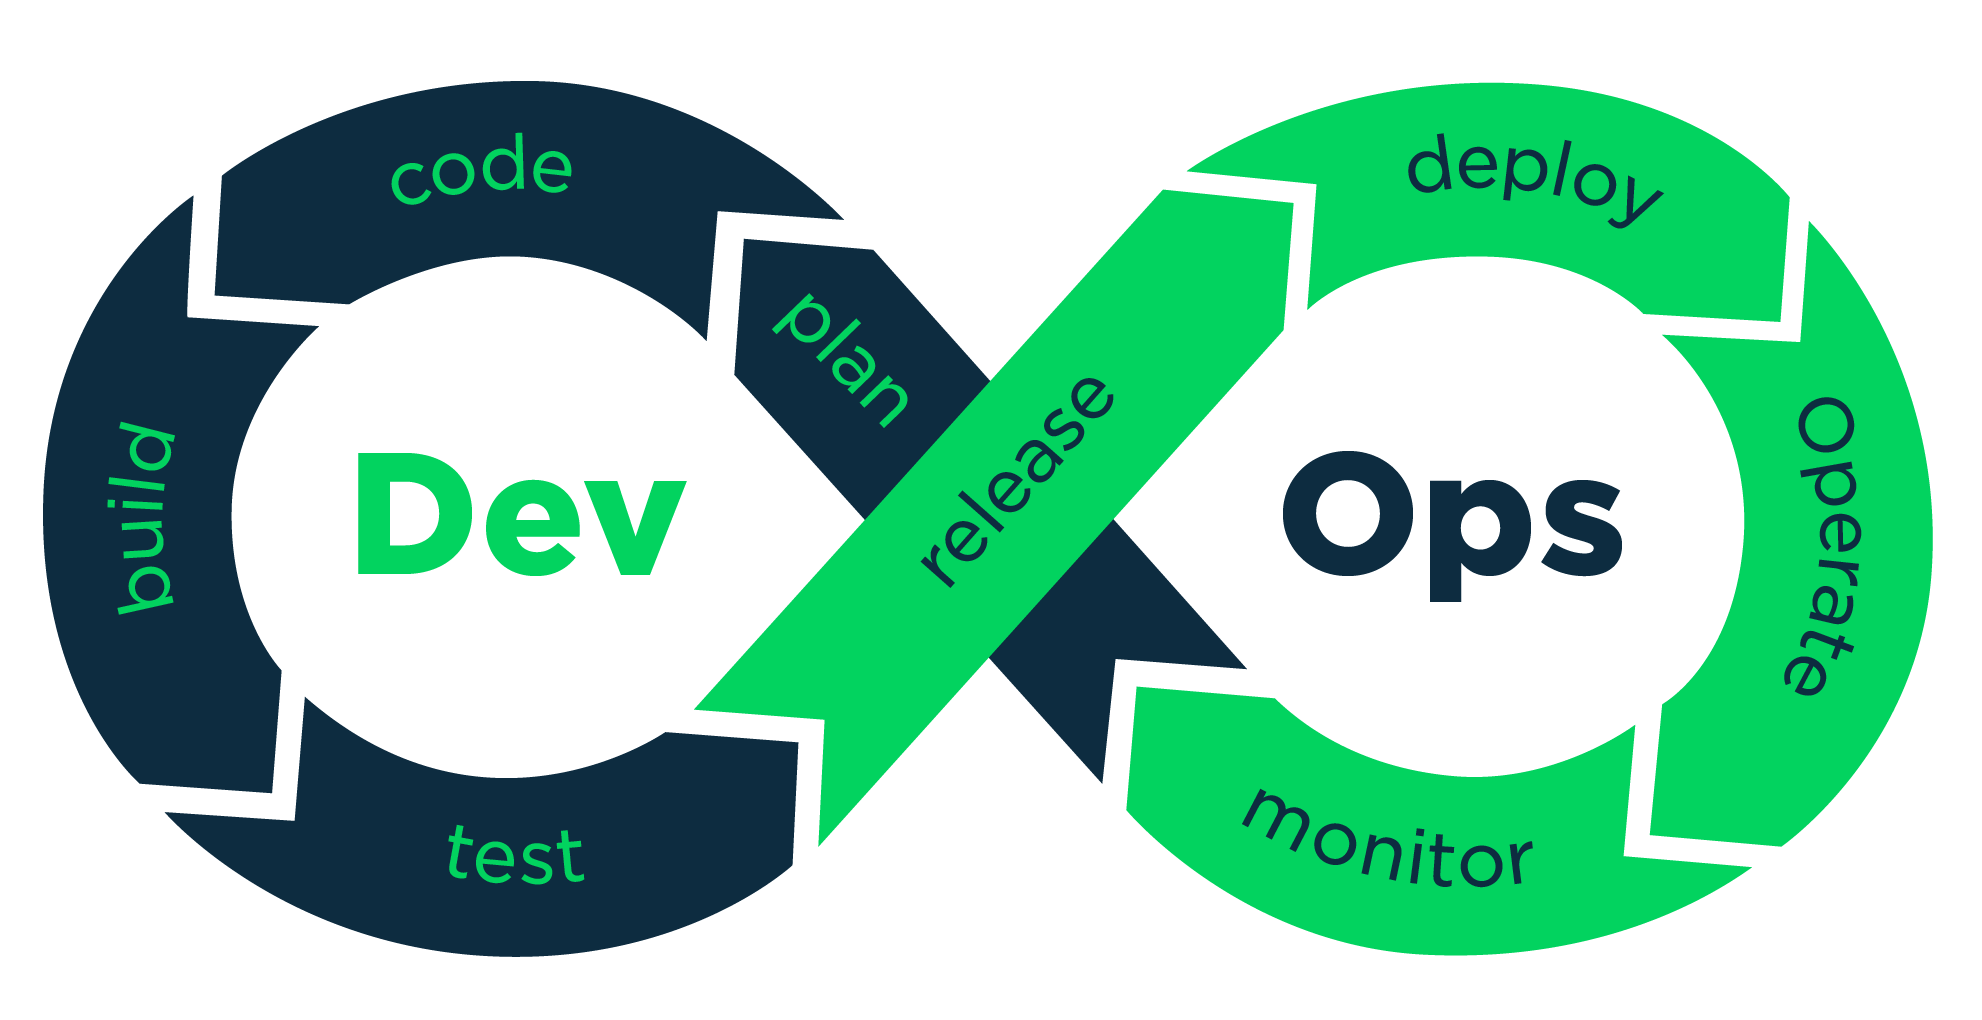
\includegraphics[width=.8\linewidth]{figures/devops-process.png}
	\caption{Le fasi della metodologia DevOps}
	\label{fig:devops-process}
\end{figure}

Il modello illustrato nella figura \ref{fig:devops-process} rappresenta il ciclo di vita del software secondo la filosofia DevOps. La disposizione delle fasi, configurata in modo da evocare il simbolo dell'infinito, simboleggia il concetto di continuità fondamentale per questa metodologia. Questo concetto è introdotto all'interno del flusso mediante un altro pilastro: l'\textit{automazione}. Grazie all'automazione, gli sviluppatori possono delegare compiti complessi o ripetitivi a sistemi esterni configurando tre componenti chiave: un evento, un'azione e il risultato atteso. Quando si verifica un evento specifico, un'entità esterna esegue un insieme di azioni predeterminate, il cui successo o fallimento viene determinato dal confronto con il risultato atteso. A livello pratico, ciò è ottenuto mediante l'utilizzo di server o più generalmente infrastrutture cloud complesse.

L'automazione dunque garantisce l'esecuzione dei processi in modo consistente e permette di concentrare le risorse del team sullo sviluppo, eliminando quindi l'intervento umano da compiti ripetitivi e passibili di errori. Una delle pratiche più diffuse, concetto rilevante della filosofia DevOps, è la pipeline di \ac{cicd}.

\paragraph{Continuous integration} La pratica della \textit{continuous integration} si concentra sull'integrazione automatica e continua delle modifiche al codice sorgente del progetto. Tipicamente, il processo si articola nei seguenti passaggi: (i) gli sviluppatori introducono nuovo codice nel progetto attraverso il software di \textit{version control}, (ii) un server acquisisce le modifiche, compila e testa l'intero progetto, (iii) una volta completato il processo, comunica agli sviluppatori l'esito delle operazioni. Questo approccio consente di individuare errori nel codice anticipatamente, garantendo stabilità e una maggiore qualità al software.

Un aspetto fondamentale è la stesura dei test: un'eccessiva copertura può rallentare il processo di integrazione. È pertanto essenziale bilanciare la copertura dei test in base alle esigenze del progetto, tenendo presente che un aumento della copertura riduce il rischio di introdurre codice difettoso.

\paragraph{Continuous delivery} La distribuzione rappresenta l'insieme di operazioni finalizzate alla consegna del software agli utenti finali. Questo processo estende l'integrazione continua e si preoccupa di garantire la disponibilità costante di un artefatto di build pronto per il rilascio. L'effettivo rilascio di una nuova versione del software può avvenire in modo automatico oppure manualmente da parte dello sviluppatore. La filosofia DevOps fornisce linee guida e non regole rigide, lasciando al team di sviluppo il compito di progettare ed integrare un flusso adeguato alle necessità del progetto.

\subsection{Un software complesso: Alchemist}\label{sec:alchemist}
Alchemist\cite{Pianini_2013} è un framework di simulazione open-source sviluppato dall'Università di Bologna, progettato per modellare elementi di programmazione pervasiva. Per comprendere l'ambito del progetto è necessario introdurre il concetto di simulazione in ambito scientifico. Per simulazione si intende un modello della realtà, costruito secondo le regole di un analista, sviluppato per consentire la valutazione dello svolgersi di una serie di eventi in un ambiente definito. Lo svolgimento di una simulazione avviene all'interno di un arco di tempo discreto suddiviso in unità di tempo predefinite conosciute come \textit{step}. Alchemist, consente di creare, osservare ed analizzare simulazioni atte a modellare interazioni tra agenti autonomi in ambienti dinamici: ossia scenari di \textit{aggregate} e \textit{nature-inspired computing}. Una rappresentazione del meta-modello, ossia le entità e relazioni configurabili, è raffigurata nella \cref{fig:alchemist-metamodel}.

\imagesource{figures/alchemist-metamodel.pdf}{https://alchemistsimulator.github.io/explanation/metamodel/}{Il meta-modello di Alchemist}{.9}{alchemist-metamodel}

\paragraph{Architettura}
Il framework è realizzato mediante linguaggi JVM-based, più precisamente Java e Kotlin, utilizzando una struttura modulare ed estendibile. Il simulatore, come già citato, è un progetto open-source, ossia distribuito sotto termini di una licenza aperta. Questa permette a tutti di osservare il codice sorgente e di contribuire allo sviluppo del progetto, coordinato da un personale responsabile del suo avanzamento. La natura open-source del progetto apre le porte a modalità di sviluppo del codice differenti rispetto a team di dimensioni ridotte. In un progetto aperto, gli utenti che contribuiscono allo sviluppo sono potenzialmente infiniti, ragion per cui l'automazione risulta determinante per mantenere un processo ordinato e controllato di integrazione e rilascio del software.

\section{Tecnologie}\label{sec:technologies}

\subsection{Gradle}

Mentre in passato la produzione di artefatti (documentazione, pacchetti, eseguibili) era delegata a script costruiti dallo sviluppatore, in un progetto di grandi dimensioni è oggigiorno essenziale avvalersi di uno strumento di \textit{build automation}. Come l'output di un programma deterministico non cambia per uno stesso input, la produzione di artefatti deve essere consistente e riproducibile riducendo al minimo l'intervento umano. 

Gradle\footnote{https://gradle.org/} è uno dei tanti strumenti disponibili, supporta diversi linguaggi di programmazione anche se risulta popolare nell'ambiente JVM come alternativa a Maven. I \textit{task} sono l'unità minima di esecuzione e rappresentano un azione: come generare un JAR, eseguire dei test o produrre la documentazione. Mediante direttive come \textit{dependsOn} è possibile creare dipendenze tra processi: Gradle orchestra l'esecuzione dei task costruendo un grafo aciclico diretto (DAG) delle dipendenze. L'esecuzione di Gradle avviene in tre fasi distinte elencate di seguito.
\begin{enumerate}
	\item \textbf{Fase di inizializzazione}: in primo luogo Gradle crea un'istanza di Settings che organizza l'architettura del progetto. Attraverso un file, di nome ``settings.gradle", lo sviluppatore stabilisce il progetto radice e tutti gli eventuali progetti figli. 
	\item \textbf{Fase di configurazione}: successivamente tutti i file di configurazione ``build\-.\-gradle" (del progetto radice e tutti i sotto-progetti) vengono analizzati per costruire il grafo dei task.
	\item \textbf{Fase di esecuzione}: infine, Gradle esegue i task richiesti considerando le dipendenze descritte nel grafo generato nella fase precedente.
\end{enumerate}

\imagesource{figures/gradle-build-lifecycle-example.png}{https://docs.gradle.org/current/userguide/build_lifecycle.html}{Esempio di inizializzazione, configurazione ed esecuzione di una build Gradle}{1}{gradle-build-lifecycle}

Un componente chiave sono i plugin, i quali consentono di estendere le funzionalità di Gradle: aggiungere nuovi task, estendere il modello con nuovi elementi ed applicare configurazioni specifiche all'intero progetto. La presenza di diversi plugin base e creati dalla comunità rende Gradle uno strumento versatile.

\subsection{GitHub Actions}

Tramite Gradle lo sviluppatore è in grado di eseguire procedure articolate come compilazione, test e dispiegamento utilizzando un semplice comando da \ac{cli}. L'invocazione di queste procedure richiede però l'intervento umano, è quindi necessario uno strumento capace di automatizzare i processi offrendo un infrastruttura resiliente e facilmente accessibile.

GitHub Actions è una piattaforma di \ac{cicd} disponibile per i repository ospitati su GitHub, che consente la configurazione ed esecuzione di pipeline personalizzate, chiamate \textit{workflow}. Questi \textit{workflow} sono flussi di processi che consistono in un insieme di \textit{job} eseguiti sequenzialmente o parallelamente all'interno di macchine virtuali denominate \textit{runner}. I workflow (\cref{fig:github-actions-example}) sono descritti in file YAML all'interno di una cartella specifica del repository. Questi file definiscono i passaggi (\textit{step}) e le azioni (\textit{action}) che il runner deve eseguire all'interno di \textit{job}, macro-processi incaricati all'esecuzione sequenziale di step.

\imagesource{figures/overview-actions-simple.png}{https://docs.github.com/en/actions/learn-github-actions/understanding-github-actions}{Sintesi dei componenti utilizzati su GitHub Actions ed esempio di un workflow}{.9}{github-actions-example}

Uno step, come citato precedentemente, rappresenta l'unità minima di esecuzione all'interno della piattaforma Actions. Le API supportano due differenti tipologie di step: (i) le azioni, ossia componenti riutilizzabili e parametrizzabili delegati all'esecuzione di una procedura specifica e (ii) i comandi shell. Le azioni possono essere create personalmente o riutilizzate attingendo da un vasto marketplace manutenuto dalla comunità.  Ad esempio, una delle azioni più diffuse e utilizzate è ``actions/checkout" [\cite{github-actions-diffusion}], la quale clona il repository del progetto nella cartella di lavoro corrente del runner.

\subsection{Package manager}

Il \textit{package management system} è un insieme di strumenti software che gestiscono i processi di installazione, aggiornamento, configurazione e rimozione di applicativi dal sistema. Tipicamente, ogni pacchetto corrisponde ad un singolo programma o applicazione, tuttavia, esistono anche applicazioni più complesse composte da numerosi pacchetti correlati. Il sistema di gestione dei pacchetti opera attraverso tre componenti principali:

\begin{itemize}
	\item Un componente a basso livello, che si occupa principalmente dell'installazione o rimozione dei pacchetti. Ricoprono questo ruolo: \textbf{rpm} il quale gestisce gli omonimi pacchetti e dpkg relativamente alla tipologia \textbf{deb}.
	\item Un componente ad alto livello, il cui compito principale è quello di fornire un'interfaccia all'utente come: \textbf{yum} per Fedora o \textbf{apt} per Debian. Si occupa inoltre di risolvere le dipendenze e gestire le sorgenti esterne (repository).
	\item I repository, ossia archivi pubblici ospitati online dalla quale l'interfaccia ad alto livello ottiene i pacchetti ed i relativi meta-dati.
\end{itemize}

\begin{figure}[H]
	\centering
	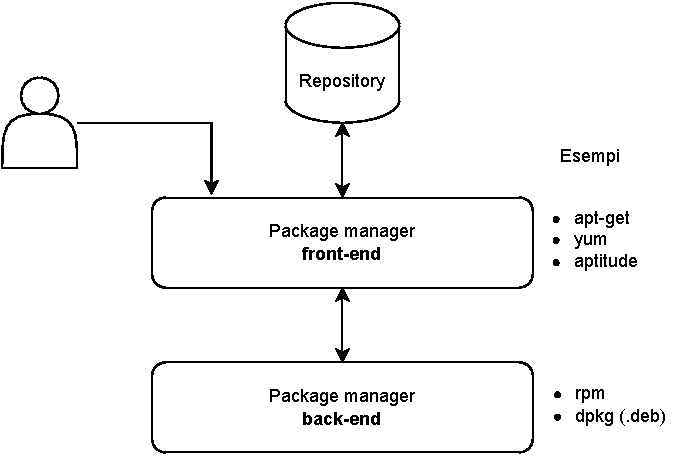
\includegraphics[width=.7\linewidth]{figures/package-managers.pdf}
	\caption{Struttura più diffusa dei sistemi di gestione di pacchetti}
	\label{fig:package-managers}
\end{figure}

L'utilizzo dei package manager fornisce diversi vantaggi nella gestione di un sistema: semplifica notevolmente il processo di aggiornamento, in quanto mediante un comando è possibile aggiornare tutti i componenti, ed allo stesso tempo, funziona da strumento di installazione capace di reperire pacchetti distribuiti in archivi online ed installarli correttamente assieme alle dipendenze richieste. 

\section{Obiettivi}
I punti discussi precedentemente hanno evidenziato l'importanza che l'automazione ricopre all'interno dello sviluppo del software. Il rilascio continuo di un applicazione è necessario per mantenere elevati standard di qualità e comporta la necessità di automatizzare questi processi per garantire la loro esecuzione in modo consistente. Inoltre, la distribuzione dell'applicativo deve avvenire mediante mezzi compatibili e diffusi per assicurare un processo di installazione semplice e funzionale agli utenti. Il package management system in questo ambito offre un approccio valido: le diverse distribuzioni Linux adoperano esso dagli albori e nei restanti due sistemi operativi, Windows e MacOs, il suo utilizzo si sta diffondendo sempre maggiormente.
\begin{figure}[htb]
	\centering
	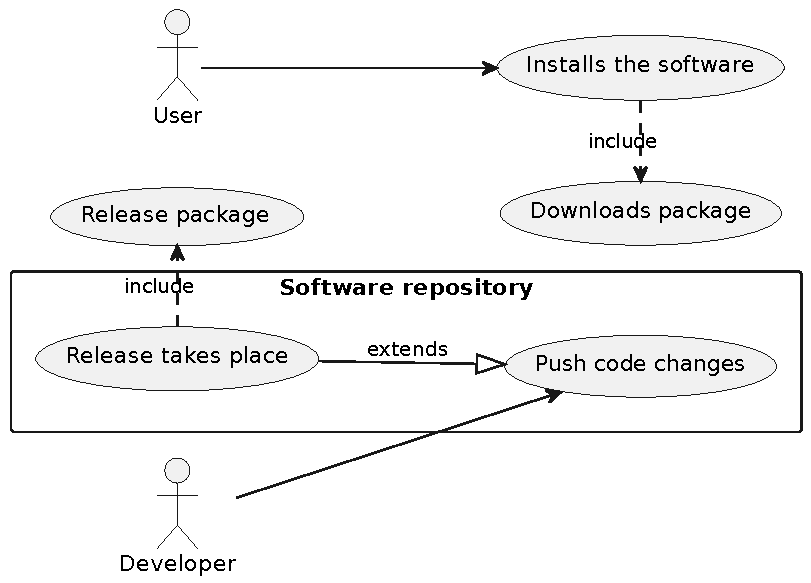
\includegraphics[width=.75\linewidth]{figures/use-case-diagram.pdf}
	\caption{Diagramma dei casi d'uso dallo sviluppatore all'utente}
	\label{fig:use-case-diagram}
\end{figure}

L'obiettivo principale dell'elaborato è quindi quello di progettare un sistema di pacchettizzazione e distribuzione del software automatico all'interno di una pipeline di integrazione e distribuzione continua. I nuovi processi devono integrarsi all'interno dell'attuale pipeline di Alchemist, estendendo le funzionalità di assemblaggio e rilascio del software. La distribuzione del pacchetto software deve avvenire per mezzo di repository pubblici diffusi, in modo da raggiungere il numero maggiore possibile di utenti; essa, inoltre, deve avvenire consistentemente nell'istante in cui una nuova versione di Alchemist viene rilasciata. La totalità dei processi integrati, inoltre, deve prevedere l'esecuzione di test all'interno del flusso, in modo da fornire un riscontro immediato nell'eventualità gli artefatti siano difettosi. Nella \Cref{fig:use-case-diagram} sono rappresentati gli scenari di utilizzo da parte degli utenti finali e degli sviluppatori di Alchemist. In particolare, lo sviluppatore introduce nuovo codice all'interno del repository del progetto e successivamente l'esecuzione della pipeline determina se è necessario il rilascio di una nuova versione. In caso di esito positivo, vengono generati i pacchetti software di installazione. Questi pacchetti, una volta distribuiti, consentiranno agli utenti di introdurre Alchemist nel proprio sistema.